\section{Introduction}

This guide is intended to guide you through the install process for the Xilinx Tools used to configure and develop snickerdoodle. This guide uses a Linux system (Ubuntu) as the platform for the download and install process. A 32 or 64-bit Linux (krtkl recommends the latest \href{http://www.ubuntu.com/download/desktop/}{LTS release from Ubuntu}) system is required to exactly follow this guide, however, the process is very similar on a Windows host. A virtual machine\sidenote{A free virtual machine hypervisor for a variety of hosts can be downloaded from \url{https://www.virtualbox.org/wiki/Downloads}} install is an excellent (and free) option for creating a Linux platform for setting up the snickerdoodle development environment. 


\section{Installing the Tools}

\subsection{Download Installer}

\infonote{To run the Xilinx tools on 64-bit systems, 32-bit runtime libraries will need to be installed. For Ubuntu systems 12.04 or newer, the \texttt{lib32z1}, \texttt{lib32ncurses5} and \texttt{lib32bz2-1.0} packages need to be installed using the \texttt{apt-get} front end for Ubuntu's packaging tool.}


\noindent
To begin downloading and installing the Xilinx tools navigate to \url{http://www.xilinx.com/support/download.html} on a web browser. 

\begin{figure*}
	\centering
	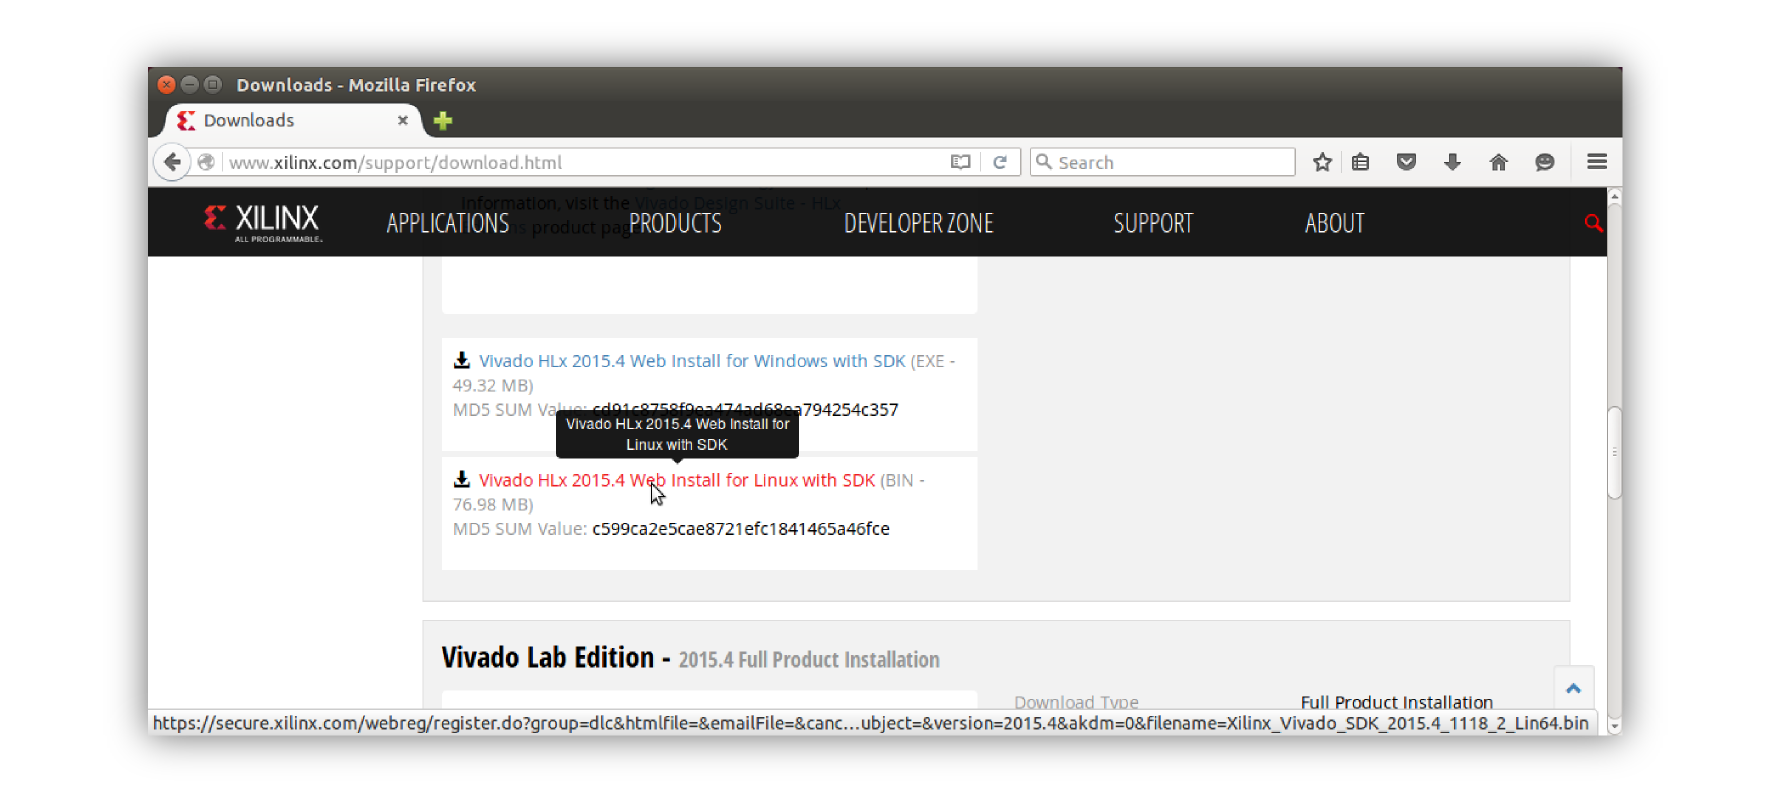
\includegraphics{images/Vivado_HLx_Download.png}
	\caption{Download Vivado and SDK Web Installer from Xilinx Website}
\end{figure*}


\subsection{Executing the Web Intaller}
\noindent
If you are using a 64-bit system, you will need to install 32-bit runtime support for the Xilinx tools using \texttt{apt-get} (on Ubuntu). Installing the runtime support can be done before or after installing the Xilinx tools. \\

\begin{lstlisting}
sudo apt-get install lib32z1 lib32ncurses5 lib32bz2-1.0
\end{lstlisting}

\margincautionnote{Make sure to execute the installer using root (\texttt{sudo}) permissions so that the installer can write to the \texttt{/opt} directory.}

~\\
\noindent
To run the web installer, first move the downloaded web installer binary from the Downloads directory. The binary needs to be given executable privelidges before running. \\

\begin{fullwidth}
\begin{lstlisting}[language=bash]
mv ~/Downloads/Xilinx_Vivado_SDK_2015.4_1118_2_Lin64.bin ..     # Move installer to home directory
cd ..                                                           
sudo chmod +x Xilinx_Vivado_SDK_2015.4_1118_2_Lin64.bin         # Modify binary permissions
sudo ./Xilinx_Vivado_SDK_2015.4_1118_2_Lin64.bin                # Execute binary
\end{lstlisting}
\end{fullwidth}


~\\
\noindent
Upon starting the installer executable, the graphical user interface (GUI) for the install process with appear. The GUI will be used to configure the install options. For most of the install options, the default values can be used. \\

\begin{figure}
	\centering
	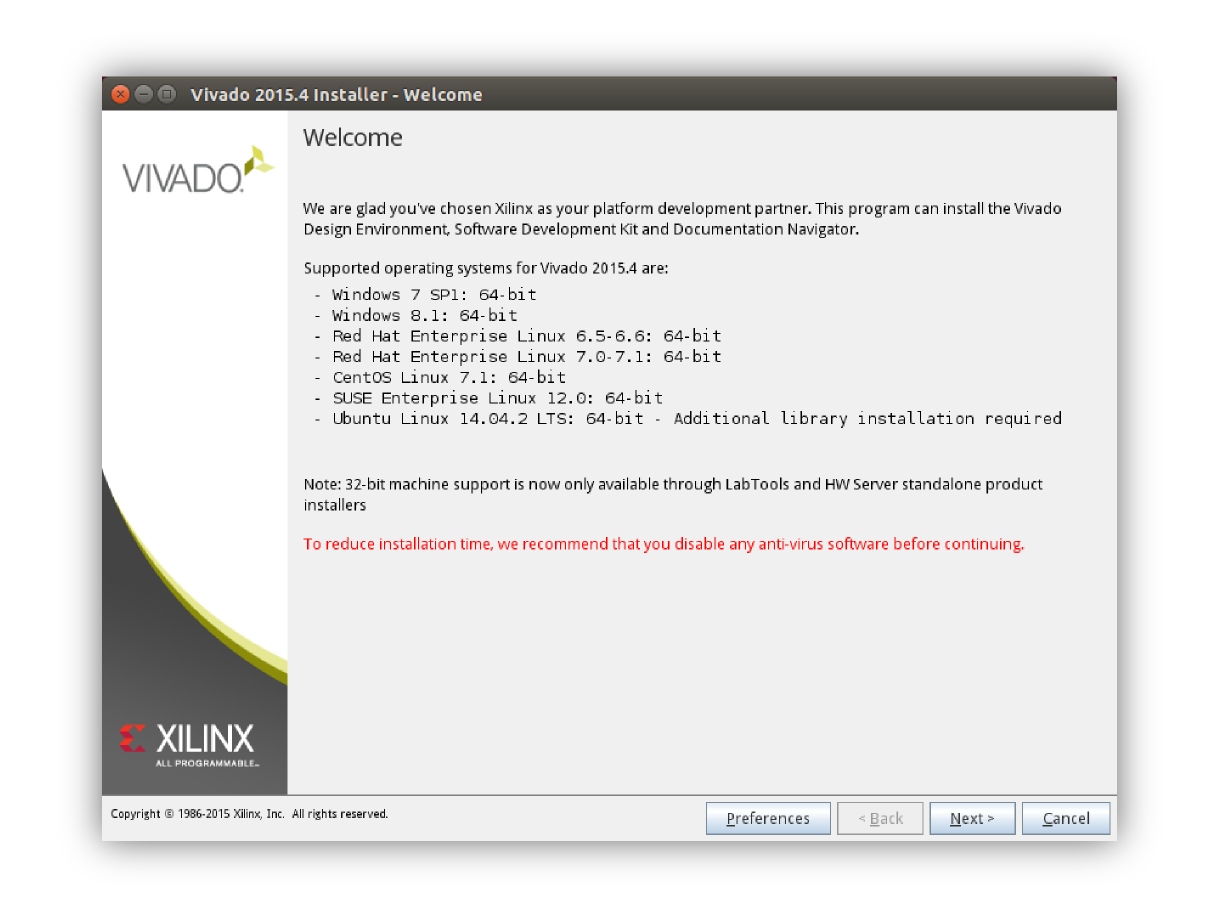
\includegraphics{images/Vivado_Installer_Welcome.png}
	\caption{Xilinx Tools Installer GUI Interface}
\end{figure}


~\\
\noindent
To start developing on snickerdoodle, the Vivado version required is the free Vivado HL WebPACK Edition. There is no version selection necessary for the SDK. The graphical Eclipse-based SDK (XSDK) will be installed by default. \\

\begin{figure}
	\centering
	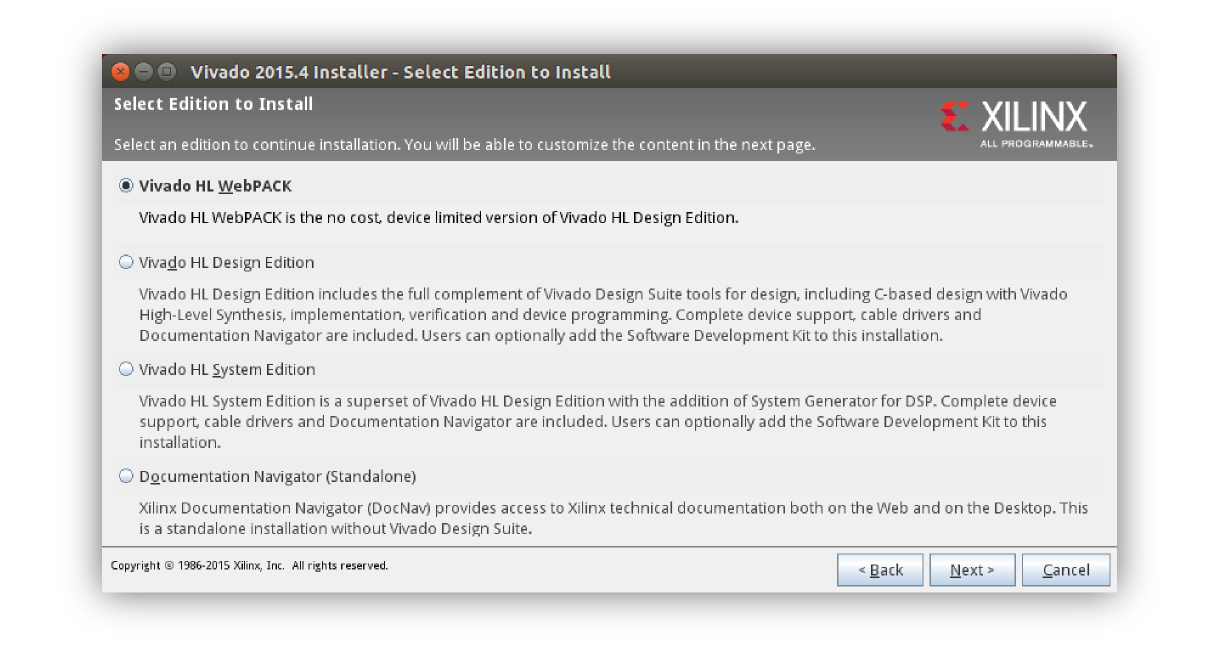
\includegraphics{images/Vivado_Installer_Edition.png}
	\caption{Selecting the Free WebPACK Vivado Edition}
\end{figure}


\noindent
The last step before the install process completes is selection of the install components including the SDK and the Xilinx Documentation Navigator (DocNav). \figref{fig:webpackconfig} shows the recommended configuration for installing the 2015.4 tools for snickerdoodle. \\

\begin{figure*}[h!]
	\centering
	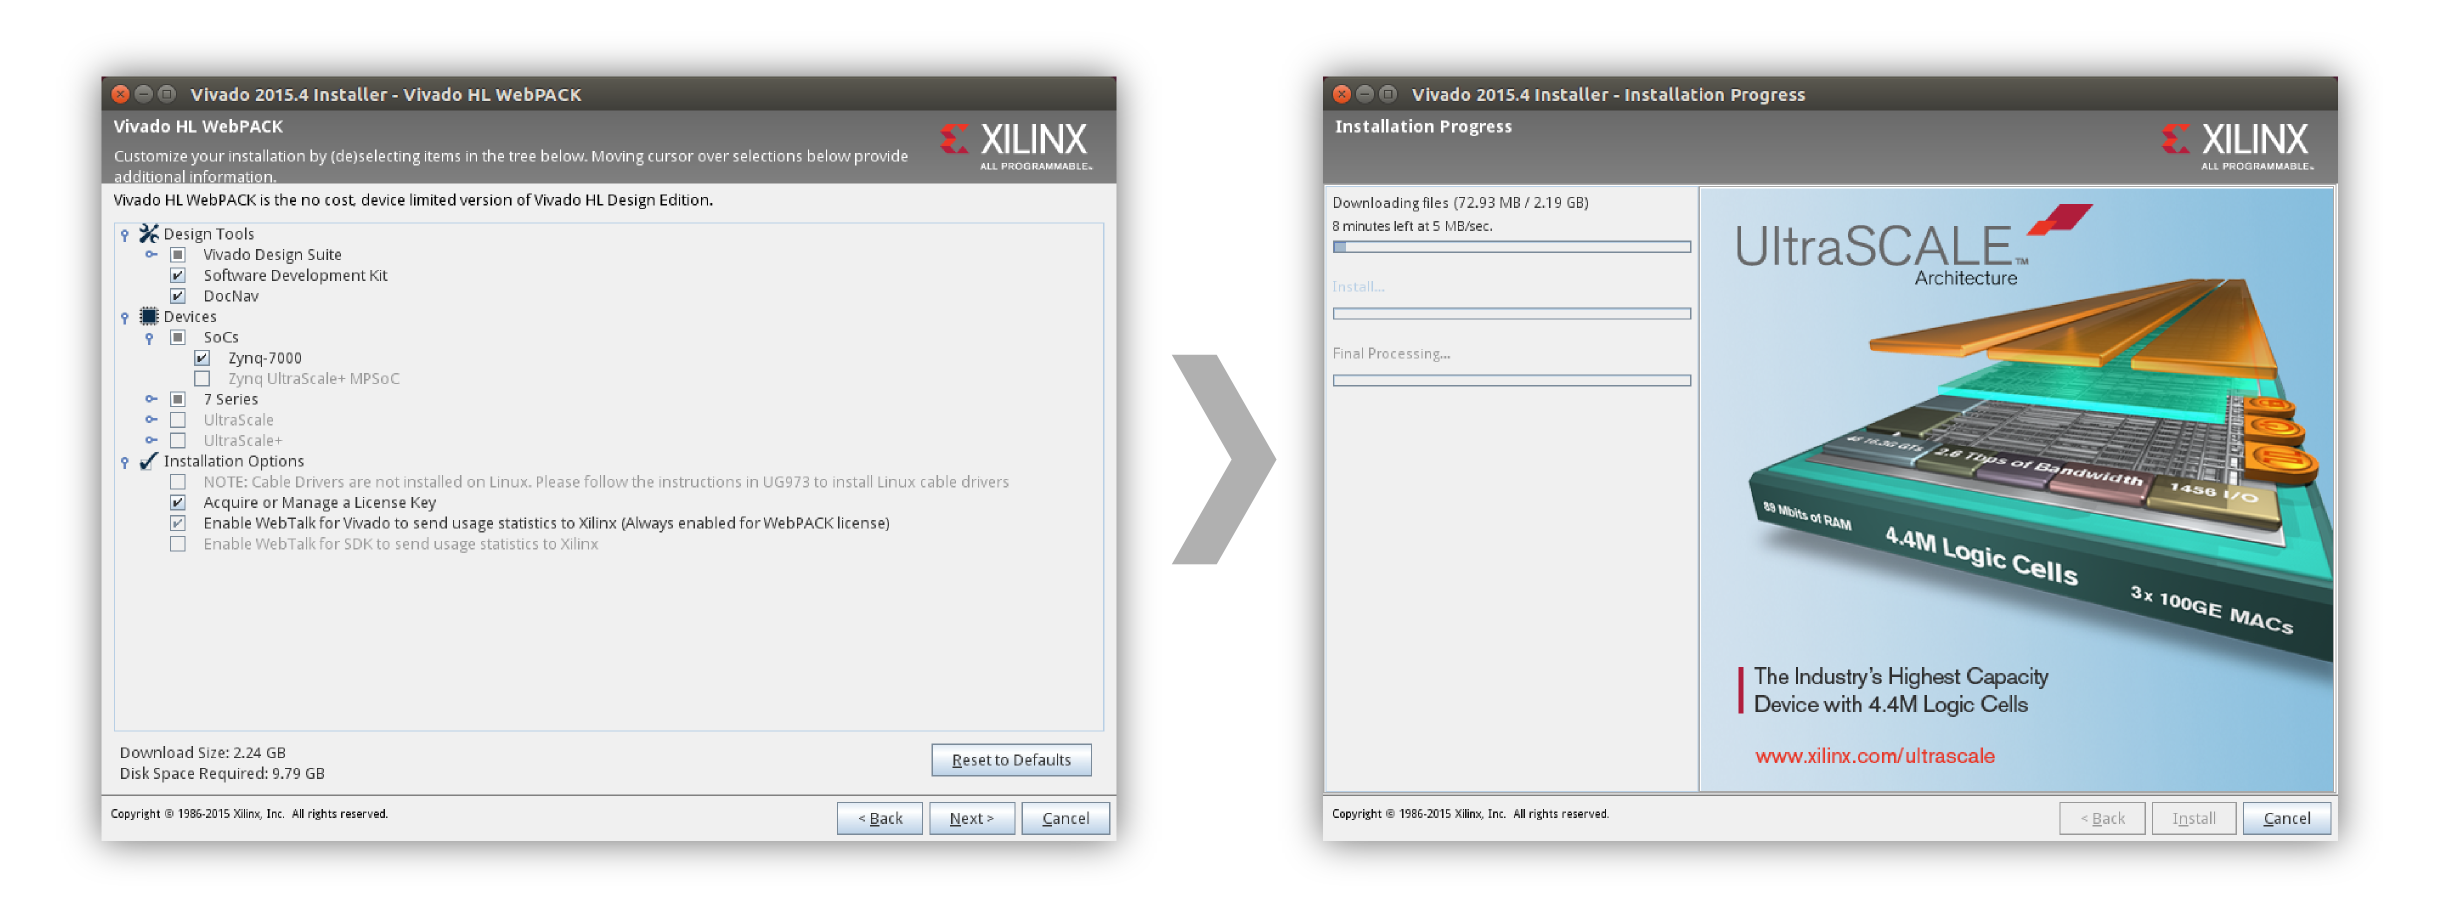
\includegraphics{images/Vivado_Installer_Webpack.png}
	\caption{Vivado HL WebPACK Install Configuration and Download/Install Progress}
	\label{fig:webpackconfig}
\end{figure*}

~\\
\noindent
Once configured, the download and install progress GUI will appear and automatically complete the installation. This will take several minutes.


\section{Licensing the Tools}

The Xilinx tools require a free account for licensing. The account will be used by the Vivado License Manger to activate the tools after they've been installed. \figref{fig:vivadolicense} shows the selection for a free WebPACK license within the Vivado License Manager. 

\begin{figure*}
	\centering
	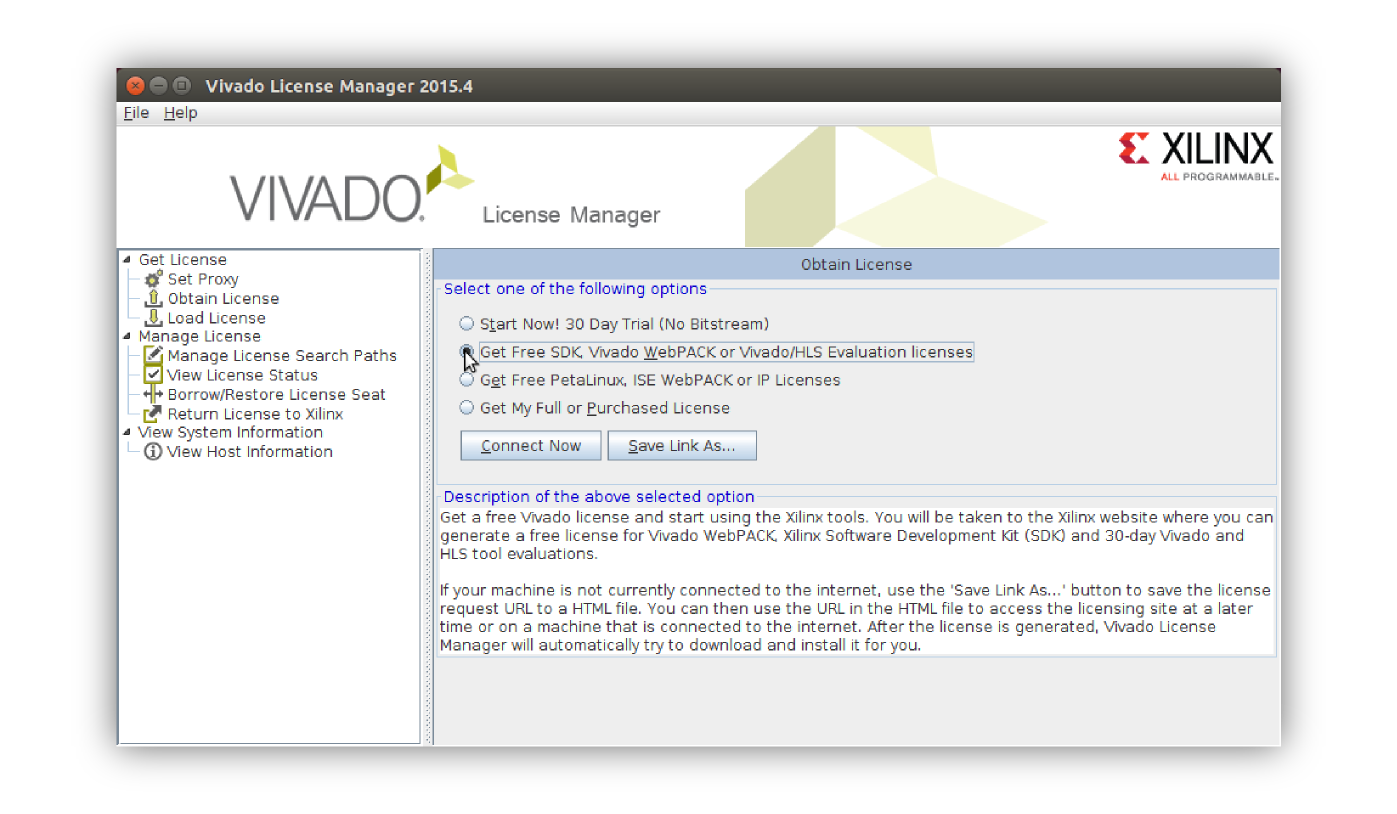
\includegraphics{images/Vivado_License_Manager.png}
	\caption{Get Free Vivado and SDK Licenses}
	\label{fig:vivadolicense}
\end{figure*}


\section{Running the Tools}

\subsection{Adding Tool Path to \texttt{\$PATH}}

The Xilinx development tools includes a set of binaries that can be accessed for a variety of development methods. To make the binaries available to tools such as GNU's \texttt{make}, the host system's \texttt{\$PATH} variable needs to be appended with the Xilinx tools directories. The tool paths are:

\begin{description}
	\item[SDK Path] \hfill \\
		\texttt{/opt/Xilinx/SDK/2015.4/bin}
	\item[Vivado Path] \hfill \\
		\texttt{/opt/Xilinx/Vivado/2015.4/bin}
	\item[DocNav Path] \hfill \\
		\texttt{/opt/Xilinx/DocNav}
	\item[ARM GCC Tools Path] \hfill \\
		\texttt{/opt/Xilinx/SDK/2015.4/gnu/arm/lin/bin}
	\item[Microblaze GCC Tool Paths] \hfill \\
	    \texttt{/opt/Xilinx/SDK/2015.4/gnu/microblaze/lin/bin} \\
		\texttt{/opt/Xilinx/SDK/2015.4/gnu/microblaze/linux\_toolchain/lin64\_be/bin} \\
		\texttt{/opt/Xilinx/SDK/2015.4/gnu/microblaze/linux\_toolchain/lin64\_le/bin}
\end{description}

\noindent
The tool paths (in this example, the SDK path) can be made temporarily available by appending the \texttt{\$PATH} variable using: \\

\begin{lstlisting}
export PATH='$PATH:/opt/Xilinx/SDK/2015.4/bin'
\end{lstlisting}

~\\
\noindent
To make the \texttt{\$PATH} specification persistent, the \texttt{/etc/environment}\sidenote{For more information on modifying the \texttt{/etc/environment} file see \url{https://help.ubuntu.com/community/EnvironmentVariables\#A.2Fetc.2Fenvironment}} file can be modified so that the tools are accessbile after restarting the host computer. The \texttt{\$PATH} variable contains a colon (\texttt{:}) sepearated list of directories to check for executable binaries. Default paths such as \texttt{/bin} and \texttt{usr/local/bin} should already be listed. \\

\noindent
After adding the tools to \texttt{\$PATH}, access to the binaries can be checked using \texttt{which} to verify the location of the binaries: \\

\begin{lstlisting}
user@ubuntu:~$ which xsdk
/opt/Xilinx/SDK/2015.4/bin/xsdk
user@ubuntu:~$ which vivado
/opt/Xilinx/Vivado/2015.4/bin/vivado
\end{lstlisting}

~\\
\noindent
Once \texttt{\$PATH} is configured to include the Xilinx tool paths, running the tools can be done by invoking the executables from a terminal. For the SDK, use \texttt{xsdk} and for Vivado, use \texttt{vivado}. The graphical interfaces will start after a short message detailing the version and SDK invocation command:

\begin{marginfigure}
	\centering
	
\includegraphics{images/SDK_Vivado_Splash.png}
	\caption[Vivado and SDK Graphical Interface Splash Screens]{Vivado and SDK Graphical Interface Splash Screens}
\end{marginfigure}


\begin{lstlisting}[%
  backgroundcolor=\color{black},
  basicstyle={\small\ttfamily\color{green}}
  ]
user@ubuntu:~$ xsdk
****** Xilinx Software Development Kit
****** SDK v2015.4 (64-bit)
  **** SW Build 1412921 on Wed Nov 18 09:44:32 MST 2015
    ** Copyright 1986-2015 Xilinx, Inc. All Rights Reserved.

Launching SDK with command /opt/Xilinx/SDK/2015.4/eclipse/lnx64.o/eclipse -vmargs -Xms64m -Xmx512m
\end{lstlisting}



